\documentclass[sigconf,nonacm]{acmart}

\setcopyright{none}
\settopmatter{printacmref=false, printccs=false, printfolios=true}
\renewcommand\footnotetextcopyrightpermission[1]{}
\pagestyle{plain}

\usepackage{booktabs}
\usepackage{tabularx}
\usepackage{graphicx}
\usepackage{amsmath}
\usepackage{balance}

\graphicspath{{figures/}}

\title{Do Global M7+ Earthquakes Occur Disproportionately After Oarfish Sightings?}

\author{Sho Akiyama}
\affiliation{%
  \institution{Independent Researcher}
  \city{Tokyo}
  \country{Japan}}
\email{contact@akiyamasho.com}

\begin{document}

\begin{abstract}
Public claims often imply that an oarfish sighting is followed by a major earthquake, but the claim is meaningful only if post-sighting earthquake rates exceed the global background rate. This paper tests that question directly for global $M \geq 7$ earthquakes with no spatial radius. The primary endpoint asks what percentage of accepted oarfish events are followed by at least one global $M7+$ earthquake within a 0--180 day prospective window, and compares that percentage with the percentage of all eligible calendar dates that are followed by a global $M7+$ earthquake in the same window. Using GBIF-indexed Regalecidae occurrences from 1980-01-01 through 2026-06-27, 461 day-dated public occurrence records reduce to 351 deduplicated oarfish events. The USGS FDSN catalog contains 659 global $M7+$ earthquakes in the same period. For the primary 0--180 day endpoint, 343 of 343 eligible oarfish events are followed by a global $M7+$ earthquake, but the overall calendar baseline is also 100.0\%; the test is saturated and provides no evidence of excess risk. In the 0--7 day sensitivity check, 93 of 351 oarfish events are followed by a global $M7+$ earthquake, or 26.5\%, compared with a 25.8\% overall calendar baseline and a same-year permutation $p=0.509$. The observed percentages do not show a statistically meaningful global $M7+$ excess after oarfish sightings.
\end{abstract}

\keywords{oarfish, Regalecidae, earthquake precursor, global temporal matching, M7 earthquakes, permutation test}

\maketitle

\section{Introduction}
The giant oarfish and related Regalecidae are rare, conspicuous deep-sea fishes. Strandings, bycatch events, and near-surface observations often receive public attention, especially in Japan where the animal is associated with the name \emph{ryugu-no-tsukai}. Folklore and media accounts sometimes interpret such appearances as earthquake warnings. Seismological agencies, however, state that deterministic earthquake prediction with exact time, place, and magnitude is not currently possible \cite{usgs_prediction,jma_prediction}.

The empirical question should be simple: after an oarfish sighting, how often does a major earthquake occur, and is that percentage higher than the overall global rate? This manuscript answers that question for global $M7+$ earthquakes. It deliberately keeps the public global-warning framing: an oarfish sighting anywhere on Earth is linked to later $M7+$ earthquakes anywhere on Earth, with no spatial radius. The confirmatory endpoint is a 0--180 day prospective window. Shorter 0--1, 0--7, and 0--90 day windows are reported only as sensitivity checks that show whether any excess appears close to the sighting date.

The distinction between an observed post-sighting percentage and an overall calendar baseline is essential. If most calendar dates are already followed by a global $M7+$ earthquake within a long window, then a high post-sighting percentage is not evidence of predictive value. The relevant comparison is therefore the probability of a global $M7+$ earthquake after an oarfish event versus the same probability after an eligible calendar date.

\begin{figure}[t]
  \centering
  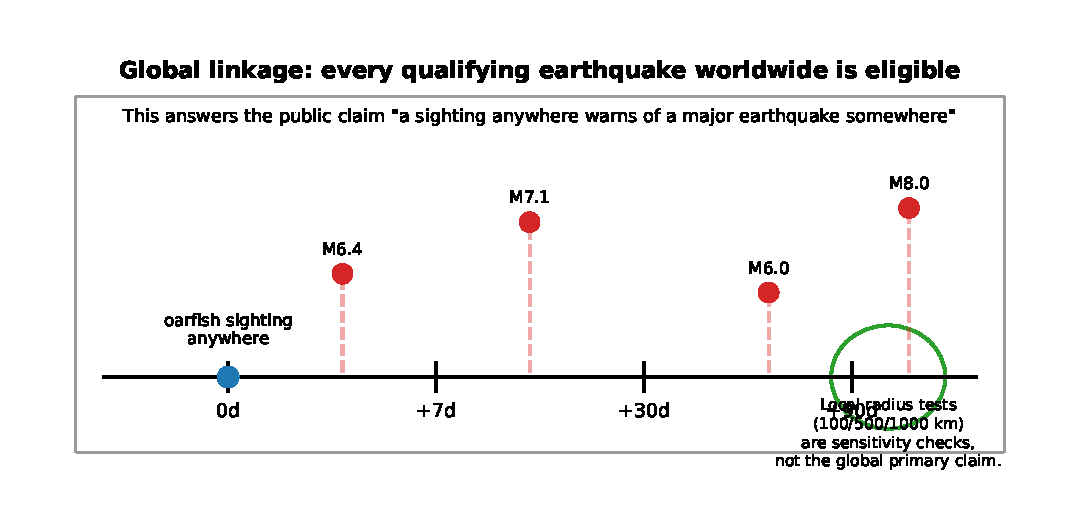
\includegraphics[width=\linewidth]{global_linkage_schematic.pdf}
  \caption{Global $M7+$ post-sighting linkage. The primary endpoint uses a 0--180 day prospective window and no spatial radius; every qualifying $M7+$ earthquake worldwide is eligible after a sighting.}
  \Description{Timeline showing one oarfish sighting date and subsequent eligible global M7 plus earthquakes within a 180 day window.}
  \label{fig:global-linkage}
\end{figure}

\section{Prior Evidence}
The strongest directly relevant peer-reviewed study is Orihara et al.'s test of Japanese folklore concerning deep-sea fish appearances and earthquakes \cite{orihara2019deepsea}. It is relevant but not oarfish-specific: the dataset contained 336 appearances of eight deep-sea fish taxa around Japan from November 1928 through March 2011. Under that historical local criterion, an earthquake with $M \geq 6$ occurring within 30 days and 100 km after an appearance, only one case qualified. The study therefore did not support a short-term local precursor claim in that setting. The present analysis asks a different question: a global, no-radius, $M7+$ temporal association after indexed Regalecidae occurrences.

\section{Data}
\subsection{Oarfish events}
The oarfish dataset was built from the GBIF Occurrence API \cite{gbif_api}. The query selected family Regalecidae, GBIF taxon key 3715, from 1980-01-01 through 2026-06-27. Records were retained when GBIF supplied a parseable day-level event date and did not mark the occurrence absent. This yielded 461 public records: 177 human observations, 219 preserved specimens, 55 material samples, 8 occurrence records, and 2 material citations.

Because the question is event-level rather than article-level or specimen-row-level, records were deduplicated before analysis. Records within three days and 10 km were treated as the same oarfish event; records without coordinates were deduplicated only on exact date, country, and locality text. The resulting analysis table contains 351 accepted oarfish events. This dataset is not every oarfish sighting ever reported; it is a reproducible public-indexed occurrence dataset, and that limitation is part of the interpretation.

\subsection{Earthquakes}
Earthquake records were acquired from the USGS FDSN Event Web Service \cite{usgs_fdsn,usgs_m7_1980_2026_query}. The query selected global earthquakes with magnitude $M \geq 7$ from 1980-01-01 through 2026-06-27 and returned 659 events. The analysis uses the USGS preferred event rows and day-level UTC origin dates.

\begin{figure}[t]
  \centering
  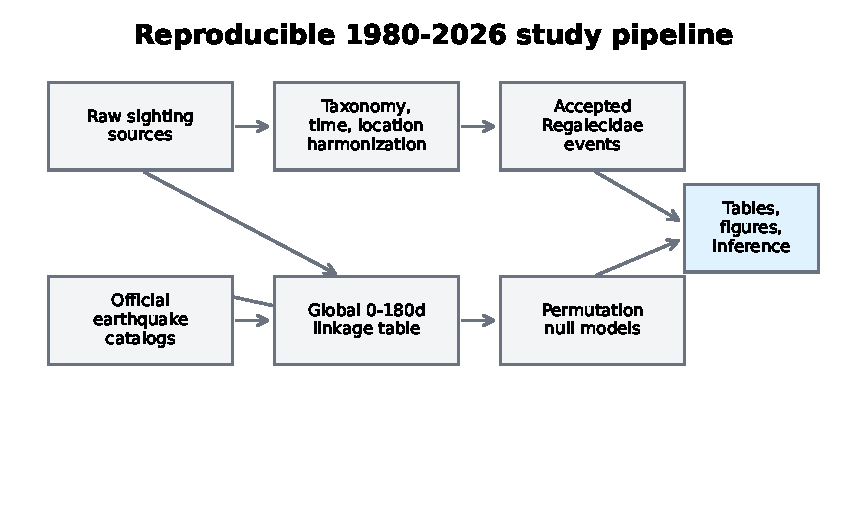
\includegraphics[width=\linewidth]{pipeline_diagram.pdf}
  \caption{Implemented analysis pipeline. GBIF Regalecidae records are converted to deduplicated oarfish events, linked prospectively to USGS global $M7+$ earthquakes, and compared with calendar and same-year permutation baselines.}
  \Description{Flow diagram from GBIF records and USGS earthquake records through deduplication, linkage, null model generation, and observed versus baseline percentages.}
  \label{fig:pipeline}
\end{figure}

\section{Methods}
\subsection{Observed post-sighting percentage}
For accepted oarfish event $i$ on day $t_i$ and prospective window $w$, the global hit indicator is
\begin{equation}
H_i(w) =
\mathbb{1}\{\exists j: m_j \geq 7,\ 0 \leq t_j - t_i \leq w\},
\end{equation}
where earthquake $j$ may occur anywhere on Earth. The observed post-sighting percentage is
\begin{equation}
\widehat{P}_{oarfish}(w) = \frac{1}{N_w}\sum_{i=1}^{N_w} H_i(w),
\end{equation}
where $N_w$ excludes right-censored oarfish events too close to 2026-06-27 to observe the full window.

\subsection{Overall calendar percentage}
The overall comparison uses the same endpoint on every eligible calendar date $d$ in the study period:
\begin{equation}
C_d(w) =
\mathbb{1}\{\exists j: m_j \geq 7,\ 0 \leq t_j - d \leq w\}.
\end{equation}
The overall global baseline is
\begin{equation}
\widehat{P}_{calendar}(w) = \frac{1}{D_w}\sum_{d=1}^{D_w} C_d(w),
\end{equation}
where $D_w$ excludes right-censored calendar dates at the end of the study period. The rate ratio is $\widehat{P}_{oarfish}(w) / \widehat{P}_{calendar}(w)$.

\subsection{Significance test}
The main uncertainty check is a same-year permutation test. For each window, every eligible oarfish date is replaced by a random eligible control date from the same calendar year, preserving the strong time trend in GBIF reporting effort. The statistic is the number of oarfish events followed by at least one global $M7+$ earthquake. The upper-tailed empirical $p$-value is
\begin{equation}
p = \frac{1 + |\{b: H^{(b)} \geq H^{obs}\}|}{B + 1},
\end{equation}
with $B=10{,}000$ permutations.

\begin{figure}[t]
  \centering
  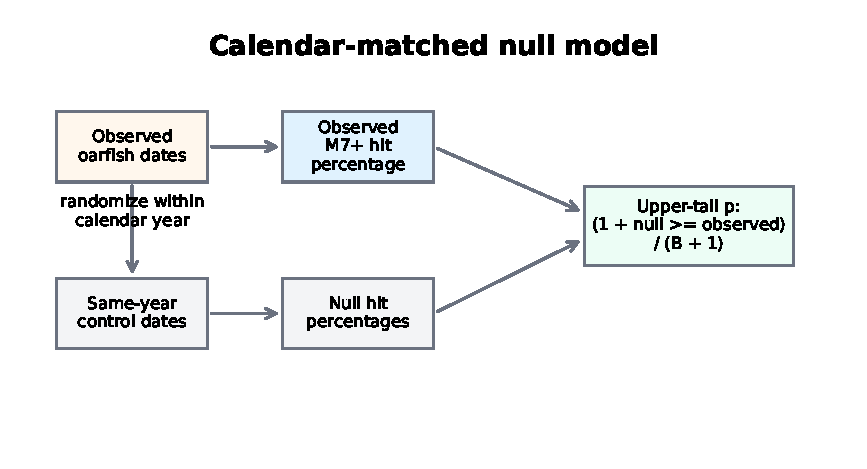
\includegraphics[width=\linewidth]{null_model_schematic.pdf}
  \caption{Calendar-matched null model. Observed post-sighting hit percentages are compared with same-year randomized control dates to test whether oarfish dates have unusually high global $M7+$ follow-on rates.}
  \Description{Diagram showing observed oarfish dates, same-year control dates, null hit percentages, and the empirical p-value formula.}
  \label{fig:null}
\end{figure}

\section{Results}
Table~\ref{tab:empirical} gives the direct answer. The primary 0--180 day endpoint is saturated: 343 of 343 eligible oarfish events, or 100.0\%, were followed by at least one global $M7+$ earthquake, but 100.0\% of eligible calendar dates were also followed by at least one global $M7+$ earthquake. This endpoint therefore has no discriminating power for the global no-radius claim in this period.

\begin{table}[t]
\caption{Observed post-oarfish global $M7+$ percentages compared with the overall global calendar baseline. The primary endpoint is 0--180 days; shorter windows are sensitivity checks.}
\label{tab:empirical}
\centering
\small
\begin{tabular}{@{}lrrrrrr@{}}
\toprule
Window & Sightings & Hits & Observed & Overall & Ratio & Perm. $p$ \\
\midrule
0--1 days & 351 & 24 & 6.8\% & 7.2\% & 0.95 & 0.722 \\
0--7 days & 351 & 93 & 26.5\% & 25.8\% & 1.03 & 0.509 \\
0--90 days & 350 & 331 & 94.6\% & 96.0\% & 0.99 & 0.970 \\
0--180 days & 343 & 343 & 100.0\% & 100.0\% & 1.00 & 1.000 \\
\bottomrule
\end{tabular}

\end{table}

Shorter windows are more informative because the overall calendar baseline is not saturated. In the 0--7 day sensitivity check, 93 of 351 oarfish events were followed by a global $M7+$ earthquake, or 26.5\%. The corresponding overall calendar percentage was 25.8\%, producing a ratio of 1.03 and a same-year permutation $p=0.509$. The 0--1 day result was 6.8\% after oarfish events versus a 7.2\% calendar baseline, with permutation $p=0.722$. The 0--90 day result was 94.6\% after oarfish events versus a 96.0\% calendar baseline, with permutation $p=0.970$.

\begin{figure}[t]
  \centering
  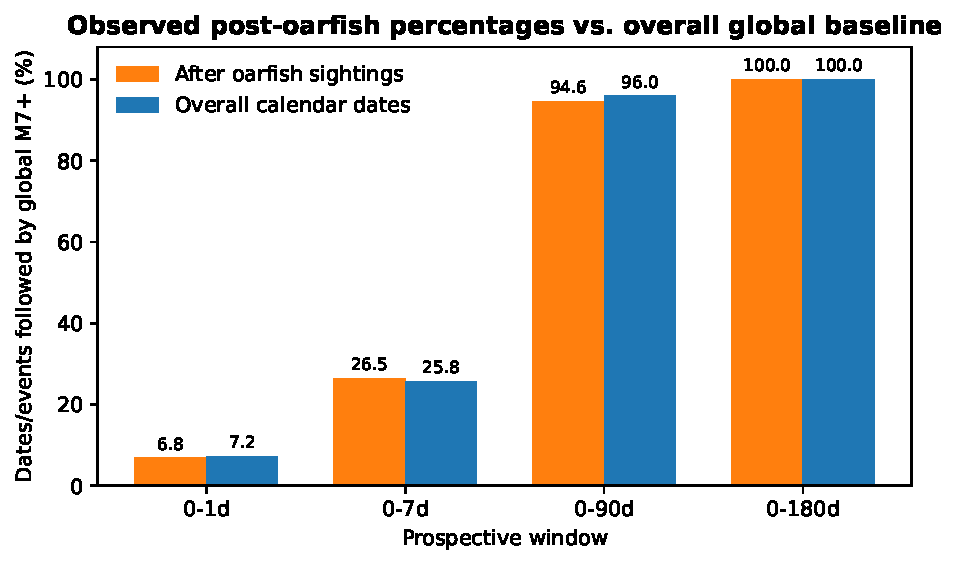
\includegraphics[width=\linewidth]{m7_observed_vs_overall.pdf}
  \caption{Observed post-oarfish percentages versus the overall calendar baseline for global $M7+$ earthquakes. The post-sighting percentages closely track the global calendar baseline rather than showing an excess after oarfish events.}
  \Description{Bar chart comparing observed post-oarfish hit percentages and overall calendar-date hit percentages across 0-1, 0-7, 0-90, and 0-180 day windows.}
  \label{fig:observed-baseline}
\end{figure}

\begin{figure}[t]
  \centering
  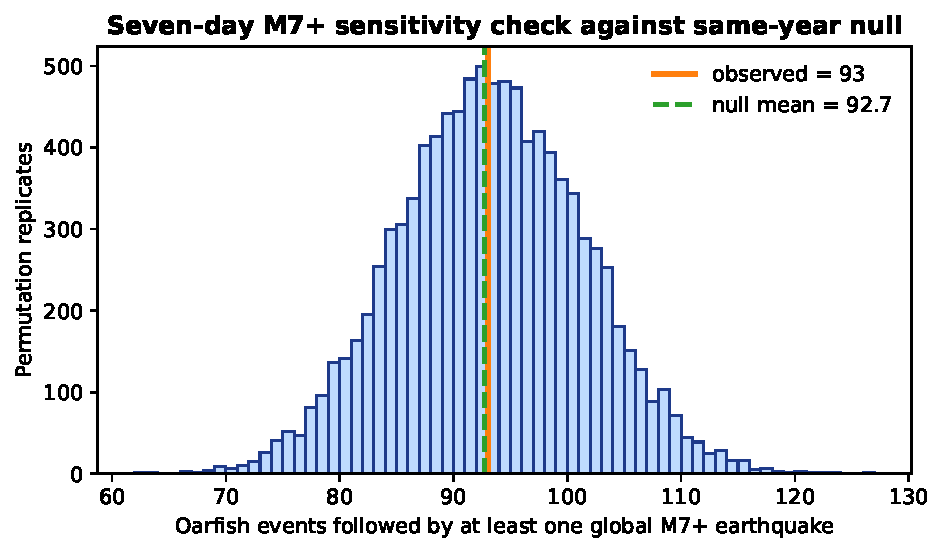
\includegraphics[width=\linewidth]{permutation_null_7d.pdf}
  \caption{Seven-day sensitivity check. The observed count of 93 oarfish events followed by a global $M7+$ earthquake is near the same-year permutation null mean and is not statistically unusual.}
  \Description{Histogram of same-year permutation hit counts for the 0-7 day window, with observed count and null mean marked.}
  \label{fig:perm7}
\end{figure}

\section{Bias and Validity}
The analysis is reproducible, but it is not immune to occurrence-data bias. GBIF records mix human observations, specimens, material samples, occurrence rows, and citations. Reporting effort changes over time, and modern citizen-science records are not sampled like older museum specimens. Deduplication also cannot perfectly distinguish two nearby oarfish from two reports of the same fish.

\begin{figure}[t]
  \centering
  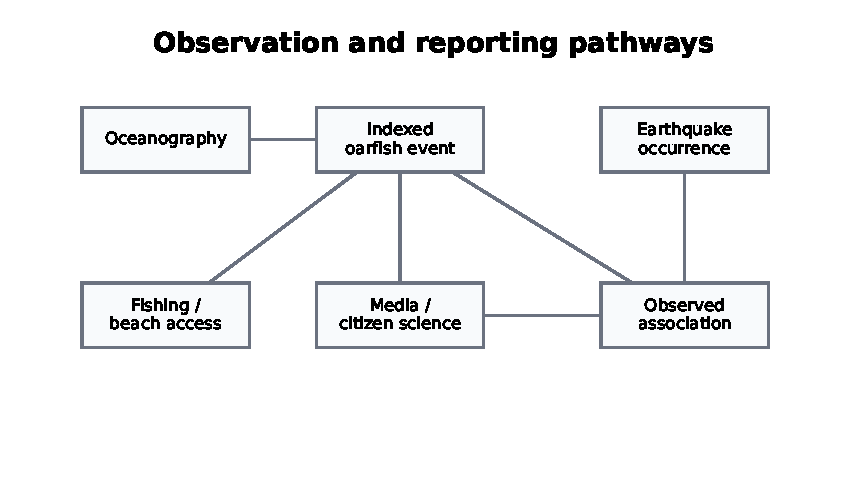
\includegraphics[width=\linewidth]{bias_dag.pdf}
  \caption{Observation and reporting pathways. Oceanographic conditions, fishing effort, beach access, and citizen-science adoption affect whether an oarfish event enters an indexed occurrence database.}
  \Description{Directed diagram linking oceanography, fishing access, media and citizen science, indexed oarfish events, earthquake occurrence, and observed association.}
  \label{fig:bias}
\end{figure}

These limitations do not explain away a positive result, because the analysis did not find one. They matter because a stronger future claim would need a fuller audited occurrence table, source-tier review, and sensitivity analyses by data source. The global no-radius endpoint also remains scientifically weak for mechanism inference: if an earthquake anywhere on Earth counts, then a high match percentage can occur even when sightings carry no predictive information.

\section{Discussion}
For the public global-warning claim, the observed percentages are not meaningfully higher after oarfish sightings than after ordinary calendar dates. The primary 0--180 day endpoint is 100.0\% after oarfish events and 100.0\% overall, so it cannot support a forecasting interpretation. The shorter windows tell the same story without saturation: the observed 0--7 day percentage is 26.5\%, close to the 25.8\% overall baseline and well inside the same-year null distribution.

The practical conclusion is that a global $M7+$ earthquake after an oarfish sighting is not surprising unless the post-sighting rate exceeds the global background rate. In this reproducible GBIF-USGS analysis, it does not. The result does not rule out every possible local biological hypothesis, but it does reject the broad global temporal claim as stated here.

\section{Conclusion}
Using public GBIF Regalecidae occurrence records and the USGS global $M7+$ earthquake catalog from 1980-01-01 through 2026-06-27, oarfish sightings do not show a statistically meaningful excess of following global $M7+$ earthquakes. The answer to the paper's core question is therefore no: in this dataset, major earthquakes are not disproportionately likely after oarfish sightings compared with the overall global calendar baseline.

\begin{acks}
This manuscript uses public biodiversity and earthquake data services. Event-level conclusions should be revisited if a fuller audited oarfish occurrence table becomes available.
\end{acks}

\balance
\bibliographystyle{ACM-Reference-Format}
\bibliography{references}

\end{document}
